% -*- coding: utf-8 -*-

\begin{chapter}{Немного истории}\label{chap:2}
% \chapter{The Historical Setting}
Наши знания о существовании океанских течений, ветров и приливов
насчитывают тысячи лет. Полинезийские мореплаватели совершали торговые
путешествия на большие расстояния в Тихом океане уже 
в 4000~до~н.~э.~\cite{Service:1996}. Пифей в 325~до~н.~э.\ исследовал Атлантику
от Италии до Норвегии. Арабские торговцы в Средние века использовали
свои знания о ветрах и течениях в Индийском океане для того, чтобы
установить торговые отношения с Китаем, а позже~--- с Занзибаром на
побережье Африки. Связь между Солнцем, Луной и приливами была
описана в Сама-веде, одном из священных писаний индуизма ведического 
периода (2000--1400~до~н.~э.)~\cite{Pugh:1987}. Некоторые океанографы, 
доверяющие только инструментальным измерениям, могли бы многому
поучиться у тех, кто зарабатывал себе на жизнь в океане.
%
% Our knowledge of oceanic currents, winds, waves, and tides goes back 
% thousands of years. Polynesian navigators traded over long distances
% in the Pacific as early as 4000 \textsc{bc} (Service, 1996). Pytheas explored 
% the Atlantic from Italy to Norway in 325 \textsc{bc}. Arabic traders used 
% their knowledge of the reversing winds and currents in the Indian Ocean to 
% establish trade routes to China in the Middle Ages and later to Zanzibar 
% on the African coast. And, the connection between tides and the 
% sun\index{sun} and moon\index{moon} was described in the Samaveda of 
% the Indian Vedic period extending from 2000 to 1400 \textsc{bc} (Pugh, 1987).
% Those oceanographers who tend to accept as true only that which has been
% measured by instruments, have much to learn from those who earned their 
% living on the ocean.

Современные европейские знания об океане начинаются с
исследовательских экспедиций Бартоломеу Диаша (1487--1488), Христофора
Колумба (1492--1494), Васко да Гама (1497--1499), Фернана
Магеллана (1519--1522) и многих других. Они заложили
основы для появления в начале XVI~века глобальных торговых маршрутов,
протянувшихся от Испании до Филиппин. Эти маршруты были основаны на
хороших знаниях о пассатах, западных ветрах и западных прибрежных
течениях в Атлантическом и Тихом океанах~\cite[стр.~192--193]{Couper:1983}.
%
% Modern European knowledge of the ocean began with voyages of discovery by
% Bartholomew Dias (1487--1488), Christopher Columbus (1492--1494), Vasco 
% da Gama (1497--1499), Ferdinand Magellan (1519--1522), and many others. 
% They laid the foundation for global trade routes stretching from Spain to 
% the Philippines in the early 16th century. The routes were based on a good 
% working knowledge of trade winds, the westerlies, and western boundary 
% currents in the Atlantic and Pacific (Couper, 1983: 192--193).

За первыми европейскими исследовательским экспедициями вскоре
последовали научные, которыми руководили, в частности,
Джеймс Кук (1728--1779) на кораблях <<Индевор>>, <<Резольюшен>> 
и~<<Эдвенчур>>,
%% англ. имена кораблей --- в предм. указатель 
%% Endeavour, Resolution, Adventure
%% википедия:Резолюшн, БСЭ: Резольюшен
%% http://slovari.yandex.ru/dict/bse/article/00039/73900.htm
%% http://ru.wikipedia.org/wiki/%D0%9A%D1%83%D0%BA_%D0%94%D0%B6%D0%B5%D0%B9%D0%BC%D1%81
%% имена людей --- тоже. Даты жизни --- тоже в указатель, чтобы не 
%% загромождать текст? И нужны ли они вообще (кому надо --- найдут)?
%% Нестыковка: в предыдущем абзаце даны даты путешествий, а в этом --- жизни?
%% Возможно, следует добавить даты жизни и остальным упомянутым исследователям:
%% Джеймс Кларк Росс (1800--1862), Джон Росс (1777--1856)
Чарльз Дарвин (1809--1882) на <<Бигле>>, сэр Джеймс Кларк Росс
%% Beagle
и сэр Джон Росс, которые проводили исследования в Арктике 
и Антарктике с кораблей <<Виктори>>, <<Изабелла>> и~<<Эребус>>, а также 
%% Victory, Isabella, Erebus
%% транслитерация "Виктори" не подтверждена источниками
Эдвард Форбс (1815--1854), изучавший вертикальное распределение жизни 
в~океанах. Другие обобщали наблюдения и строили на их основе различные карты,
так, Эдмунд Галлей картировал пассаты и~муссоны, 
а Бенджамин Франклин нанёс на карту Гольфстрим.
%% Эдмунд Галлей (1656--1742), Бенджамин Франклин (1706--1790)
%
% The early European explorers were soon followed by scientific voyages of
% discovery led by (among many others) James Cook (1728--1779) on the
% \textit{Endeavour}, \textit{Resolution}, and \textit{Adventure}, 
% Charles Darwin (1809--1882) on the \textit{Beagle}, Sir James Clark Ross 
% and Sir John Ross who surveyed the Arctic and Antarctic regions from the 
% \textit{Victory}, the \textit{Isabella}, and the \textit{Erebus}, and Edward 
% Forbes (1815--1854) who studied the vertical distribution of life in the ocean. 
% Others collected oceanic observations and produced useful charts, including 
% Edmond Halley who charted the trade winds and monsoons and Benjamin Franklin 
% who charted the Gulf Stream\index{Gulf Stream!mapped by Benjamin Franklin}.

Медленные корабли XIX и~XX~веков уступили в конце XX~века дорогу
спутникам, дрейфующим буям и другим автоматическим приборам. 
Сейчас спутники исследуют океаны, атмосферу и сушу. Тысячи дрейфующих буев
ведут наблюдения на глубинах до двух километров. Полученные с их помощью
данные обрабатываются при помощи численных моделей и позволяют изучать Землю как
единую систему. Впервые в истории науки мы получили возможность узнать, 
как биологические, химические и физические системы взаимодействуют между 
собой и влияют на окружающую среду.
%
% Slow ships of the 19th and 20th centuries gave way to satellites, drifters, 
% and autonomous instruments  toward the end of the 20th century. Satellites 
% now observe the ocean, air, and land. Thousands of drifters observe the 
% upper two kilometers of the ocean. Data from these systems, when fed into 
% numerical models allows the study of earth as a system. For the first time, 
% we can study how biological, chemical, and physical systems interact 
% to influence our environment.

\begin{section}{Определения}
% \section{Definitions}
Долгая история изучения океана привела к появлению различных
специализированных дисциплин, каждая из которых обладает своими
собственными интересами и терминологией. Среди этих дисциплин наиболее важны
следующие:
%
% The long history of the study of the ocean has led to the development of
% various, specialized disciplines each with its own interests and
% vocabulary. The more important disciplines include:

\begin{description}
\item[Океанография] занимается изучением океана как среды. Целью этой
науки является получение количественного описания океана, достаточного
для того, чтобы с некоторой достоверностью предсказывать его будущее
состояние.
%
% \textit{Oceanography} is \index{oceanography|textbf}the study of the ocean, 
% with emphasis on its character as an environment. The goal is to obtain 
% a description sufficiently quantitative to be used for predicting the future 
% with some certainty.


\item[Геофизика] изучает физику Земли.
%
% \textit{Geophysics} is \index{geophysics|textbf}the study of the physics 
% of the earth.

\item[Физическая океанография] изучает физические характеристики и
динамику океанов. Основными интересами этой науки являются
взаимодействие океана с атмосферой, тепловой баланс океана,
формирование водных масс, течения и процессы в прибрежных
областях. Многими физическая океанография рассматривается как раздел
геофизики.
%
% \textit{Physical Oceanography} is \index{physical oceanography|textbf}the 
% study of physical properties and dynamics of the ocean. The primary interests 
% are the interaction of the ocean with the atmosphere, the oceanic heat budget, 
% water mass formation, currents, and coastal dynamics. Physical Oceanography 
% is considered by many to be a subdiscipline of geophysics.

\item[Геофизическая гидродинамика] изучает динамику движения жидкости
%% не гидромеханика, а гидродинамика?
%% http://www.multitran.ru/c/m.exe?CL=1&l1=1&s=fluid+dynamics
%% http://ru.wikipedia.org/wiki/%D0%93%D0%B8%D0%B4%D1%80%D0%BE%D0%BC%D0%B5%D1%85%D0%B0%D0%BD%D0%B8%D0%BA%D0%B0
%% т.к. речь идет о динамике --- то "гидродинамика"
в масштабах, в которых ощущается влияние вращения Земли. Метеорология и
%% Возможная неточность перевода. М.б. речь идет о конкретных гидродинамических 
%% явлениях, вызываемых вращением Земли?
океанография используют геофизическую гидродинамику для расчёта полей
планетарных течений.
%
% \textit{Geophysical Fluid Dynamics} is \index{geophysical fluid dynamics|textbf}
% the study of the dynamics of fluid motion on scales influenced by the 
% rotation of the earth. Meteorology and oceanography use geophysical fluid 
% dynamics to calculate planetary flow fields.

\item[Гидрография] занимается составлением морских карт, таких как
карты глубины океана, течений, полей плотности в океане и приливов.
%
% \textit{Hydrography} is \index{hydrography|textbf}the preparation of nautical 
% charts, including charts of ocean depths, currents, internal density field 
% of the ocean, and tides.

\item[Науки о Земле] изучают Землю как единую систему, в состав 
%% http://en.wikipedia.org/wiki/Earth_System_Science
%% http://ru.wikipedia.org/wiki/%D0%9D%D0%B0%D1%83%D0%BA%D0%B8_%D0%BE_%D0%97%D0%B5%D0%BC%D0%BB%D0%B5
%% согласно этим статьям, нет конкретно такой науки, это общий термин для
%% всех наук о Земле?
которой входит множество взаимодействующих подсистем, таких как океан, 
атмосфера, криосфера и биосфера.%
\remark{Научная дисциплина <<Earth-system Science>> пока не имеет точного 
аналога в русскоязычной номенклатуре; как следствие, общепринятый перевод её
названия также отсутствует.} 
Отдельным важным объектом исследований
служат изменения, происходящие в этих подсистемах под влиянием деятельности
человечества.
%
% \textit{Earth-system Science} is \index{earth-system science|textbf}the study 
% of earth as a single system comprising many interacting subsystems including 
% the ocean, atmosphere, cryosphere, and biosphere, and changes in these 
% systems due to human activity.
\end{description}
\end{section}

\begin{section}{Периоды исследований океана}
% \section{Eras of Oceanographic Exploration}
Исследование океана можно условно разделить на различные периоды~\cite{Wust:1964}. 
Рассмотрим эту классификацию, расширив её до конца XX~века:
%
% The exploration \index{oceanography!eras of exploration|(}of the sea can be 
% divided, somewhat arbitrarily, into various eras (Wust, 1964). I have 
% extended his divisions through the end of the 20th century.
\begin{enumerate}
\item  
Период поверхностной океанографии: с древнейших времён до~1873. 
Систематизация наблюдений за ветрами,
течениями, волнами, температурой и другими явлениями, поддающимися
наблюдению с палубы корабля. Известными примерами достижений той эпохи 
служат карты пассатов, составленные Галлеем, карта Гольфстрима Франклина 
и книга Мэтью Фонтейна Мори <<Физическая география моря>>.
%% Мэтью Фонтейн Мори (1806--1873)
%% (Physical Geography for the Sea.) --- англ. книгу в индекс???
%% Полное название другое? The physical geography of the sea and its meteorology
%% http://bse.sci-lib.com/article078157.html
%
% \vitem Era of Surface Oceanography: Earliest times to 1873. The era is 
% characterized by systematic collection of mariners' observations of winds, 
% currents, waves, temperature, and other phenomena observable from the deck 
% of sailing ships. Notable examples include Halley's charts of the trade 
% winds, Franklin's map of the 
% Gulf Stream\index{Gulf Stream!mapped by Benjamin Franklin}, and 
% Matthew Fontaine Maury's \textit{Physical Geography of the Sea}.

\item
Период глубоководных исследований: 1873--1914.
Различные по значимости океанографические экспедиции, цель 
которых~--- выяснение поверхностных и глубинных характеристик океана возле
колониальных земель. Важнейший пример~--- экспедиция
<<Челленджера>> (рис.~\ref{fig:Fig2-1}), но можно назвать также экспедиции 
<<Газели>> и~<<Фрама>>.
%
% \vitem Era of Deep-Sea Exploration: 1873--1914. Characterized by a few, 
% wide-ranging oceanographic expeditions to survey surface and subsurface 
% conditions, especially near colonial claims. The major example is the 
% \textit{Challenger} Expedition (figure 2.1), but also the \textit{Gazelle}
% and \textit{Fram} Expeditions.

\begin{figure}[th]
\includegraphics{pics/Fig2-1}
\caption{Пример экспедиции периода глубоководных исследований. Путь 
<<Челленджера>> (Великобритания) в ходе экспедиции 1872--1876~гг. Wust (1964).}
\label{fig:Fig2-1}
\end{figure}
%
% \begin{figure}[t!]
% \includegraphics{Fig2-1}
% \centering
% \footnotesize
% Figure 2.1 Example from the era\rule{0pt}{3ex} of deep-sea exploration: Track of
% H.M.S. \textit{Challenger}\\ during the British Challenger Expedition
% 1872--1876. After Wust (1964).
%
% \label{fig:Fig2-1}
% \vspace{-3ex}
% \end{figure}

\item
Период национальных систематических исследований: 1925--1940.
%% "Детальное изучение колониальных областей." --- авторская неточность (?)
Как примеры можно привести изучение Атлантики <<Метеором>> 
(рис.~\ref{fig:Fig2-2}) и экспедицию <<Дискавери>>.
%
% \vitem Era of National Systematic Surveys: 1925--1940. Characterized by 
% detailed surveys of colonial areas. Examples include \textit{Meteor} surveys 
% of the Atlantic (figure 2.2), and the \textit{Discovery} Expeditions.

\begin{figure}[t!]
\makebox[121mm][c]{\includegraphics{pics/Fig2-2}}
\caption{Пример экспедиции периода национальных систематических исследований.
Путь НИС <<Метеор>> (Германия)~\cite{Wust:1964}.}
\label{fig:Fig2-2}
\end{figure}
%
% \begin{figure}[t!]
% \makebox[121mm] [c] {\includegraphics{Fig2-2}}
% \centering
% \footnotesize
% Figure 2.2 Example of a survey from the era of national\rule{0pt}{3ex} systematic
% surveys. Track of the R/V \textit{Meteor} during the German Meteor Expedition. Redrawn from
% Wust (1964).
% 
% \label{fig:Fig2-2}
% \vspace{-3ex}
% \end{figure}

\item
Период новых методов: 1947--1956. Долговременные
исследования с использованием новых инструментов (рис.~\ref{fig:Fig2-3}). Как
пример можно привести сейсмическое изучение Атлантики с судна <<Вема>>, в
результате которого Б.~Хейзеном были составлены карты морского дна.
%% Heezen -- Хейзен/Хизен: http://slovari.yandex.ru/dict/bse/article/00086/39500.htm
%% Б.~Хейзен (1924--1977)
%
% \vitem Era of New Methods: 1947--1956. Characterized by long surveys using 
% new instruments (figure 2.3). Examples include seismic surveys of
% the Atlantic by \textit{Vema} leading to Heezen's maps of the sea floor.

\begin{figure}[t!]
\makebox[121 mm] [c] {\includegraphics{pics/Fig2-3}}
\caption{Пример экспедиции периода новых методов: путь НИС <<Атлантис>>
(Океанографический институт в Вудсхоле)~\cite{Wust:1964}.}
\label{fig:Fig2-3}
\end{figure}
%
% \begin{figure}[t!]
% \makebox[121 mm] [c] {\includegraphics{Fig2-3}}
% \centering
% \footnotesize
% Figure 2.3  Example from the era of new \rule{0pt}{4ex}methods. The cruises of
% the R/V \textit{Atlantis} out of Woods Hole Oceanographic Institution. After Wust
% (1964).
% 
% \label{fig:Fig2-3}
% \vspace{-3ex}
% \end{figure}

\item
Период международной кооперации: 1957--1978.
Многонациональные исследования океана и происходящих в нем процессов.
Примеры: Программа Атлантический Полярный Фронт
(Atlantic Polar Front Program), рейсы NORPAC, рейсы в ходе
Международного геофизического года и Международной декады изучения
океана (рис.~\ref{fig:Fig2-4}), исследования с одновременным участием 
нескольких десятков кораблей~--- эксперименты MODE, POLYMODE, NORPAX и~JASIN.
%
% \vitem Era of International Cooperation: 1957--1978. Characterized by
% multinational surveys of ocean and studies of oceanic processes. Examples
% include the Atlantic Polar Front Program, the \textsc{norpac} cruises,
% the International Geophysical Year cruises, and the International Decade
% of Ocean Exploration (figure 2.4). Multiship studies of oceanic processes
% include \textsc{mode}, \textsc{polymode}, \textsc{norpax},
% and \textsc{jasin} experiments.

\begin{figure}[t!]
\includegraphics{pics/Fig2-4}
\caption{Пример экспедиций периода международной кооперации:
измерения, проведённые в ходе Атлантической программы Международного 
геофизического года 1957--1959~гг.~\cite{Wust:1964}.}
\label{fig:Fig2-4}
\end{figure}
%
% \begin{figure}[t!]
% \includegraphics{Fig2-4}
% \centering
% \footnotesize
% Figure 2.4  Example from the era of international cooperation
% \rule{0pt}{3ex}. Sections measured by the International
% Geophysical Year Atlantic Program 1957-1959. After Wust (1964).
% 
% \label{fig:Fig2-4}
% \vspace{-3ex}
% \end{figure}

\item
Эра спутников: 1978--1995. Глобальное
изучение океанических процессов из космоса. Примеры: Seasat, 
NOAA~6--10, NIMBUS-7, Geosat, Topex/Poseidon, ERS-1 и~ERS-2.
%
% \vitem Era of Satellites: 1978--1995. Characterized by global surveys of 
% oceanic processes from space. Examples include Seasat, \textsc{noaa} 6--10, 
% \textsc{nimbus}--7, Geosat\index{Geosat}, 
% Topex/\-Poseidon\index{Topex/Poseidon}, and \textsc{ers}--1 \& 
% 2\index{ERS satellites}. 

\item
Эра изучения Земли как системы: 1995--. Изучение в глобальных масштабах
взаимодействия биологических, химических и физических
процессов в океане, атмосфере и на суше с использованием численных моделей
и входных данных для них, полученных как in situ (то есть, непосредственно 
в океане), так и из космоса. В случае океана это
World Ocean Circulation Experiment (WOCE) (рис.~\ref{fig:wocesurvey}) 
и Topex/Poseidon (рис.~\ref{fig:Fig2-6}), Join Global
Ocean Flux Study (JGOFS), Global Ocean Data Assimilation Experiment (GODAE),
а также спутники SeaWiFS, Aqua и~Terra.
%% проверить, что в самом деле спутники, а что --- названия экспериментов
%
% \vitem Era of Earth System Science: 1995-- Characterized by global studies 
% of the interaction of biological, chemical, and physical processes in the 
% ocean and atmosphere and on land using \textit{in situ} \index{in situ|textbf} 
% (which means from measurements made in the water) and space data in numerical 
% models. Oceanic examples include the World Ocean Circulation Experiment 
% (\textsc{woce})\index{World Ocean Circulation Experiment} (figure 2.5) 
% and Topex/Poseidon (figure 2.6), the Joint Global Ocean Flux 
% Study \index{oceanography!eras of exploration|)} (\textsc{jgofs}), 
% the Global Ocean Data Assimilation Experiment (\textsc {godae}), 
% and the SeaWiFS, Aqua, and Terra satellites.
\end{enumerate}

\begin{figure}[t!]
\includegraphics{pics/wocesurvey}
\caption{Эксперимент по исследованию циркуляции мирового океана (WOCE):
пути НИС, осуществлявших одновременное глобальное исследование мирового океана
(по данным World Ocean Circulation Experiment).}
\label{fig:wocesurvey}
\vspace{-3ex}
\end{figure}
%
% \begin{figure}[t!]
% \includegraphics{wocesurvey}
% \centering
% \footnotesize
% Figure 2.5 World Ocean\index{World Ocean Circulation Experiment} Circulation
% Experiment:\rule{0pt}{4ex} Tracks of research ships making a one-time global 
% survey of the ocean of the world. From World Ocean Circulation Experiment.
%
% \label{fig:wocesurvey}
% \vspace{-3ex}
% \end{figure}

\begin{figure}[b!]
\makebox[121mm][c]{\includegraphics{pics/Fig2-6}}
\caption{Пример периода изучения Земли, как системы:
трассы спутника Topex/Poseidon над Тихим океаном за период 10~дней
(по данным Topex/Poseidon Project).}
\label{fig:Fig2-6}
\end{figure}
%
% \begin{figure}[b!]
% \vspace{-1ex}
% \makebox[121mm][c]{\includegraphics{Fig2-6}}
% \centering
% \footnotesize
% Figure 2.6 Example \rule{0mm}{3ex}from the era of satellites.
% Topex/Poseidon\index{Topex/Poseidon!ground tracks} tracks in the 
% Pacific\\Ocean during a 10-day
% repeat of the orbit. From Topex/Poseidon Project.
% 
% \label{fig:Fig2-6}
% %\vspace{-3ex}
% \end{figure}
\end{section}

\begin{section}{Вехи в понимании океана}
% \section{Milestones in the Understanding of the Ocean}
Что же удалось узнать об океане в ходе исследовательских программ и
экспедиций, упомянутых в предыдущем разделе? Перечислим некоторые ключевые
достижения, начиная с XVII~в. Сначала прогресс
был очень медленным. Первые простые, но очень важные в перспективе
наблюдения были сделаны учёными, которые не считали себя океанографами, 
если такой термин в те времена вообще существовал. 
В дальнейшем пришла пора более детальных описаний и океанографических 
экспериментов, проделанных учёными, специализирующимися
именно на изучении океана. 
%
% What have all these programs and expeditions taught us about the ocean?
% Let's look at some milestones in our ever increasing understanding of 
% the ocean beginning with the first scientific investigations of the 17th 
% century. Initially progress was slow. First came very simple observations 
% of far reaching importance by scientists who probably did not consider 
% themselves oceanographers, if the term even existed. Later came more detailed 
% descriptions and oceanographic experiments by scientists who specialized in 
% the study of the ocean.

\begin{description}
\item[1685] Эдмунд Галлей опубликовал результаты проведенного
изучения океанской системы ветров и течений в работе <<Историческая оценка 
пассатов и муссонов, наблюдаемых в морях между и вблизи тропиков, 
и попытка установить физическую причину возникновения
названных ветров>> (<<An Historical Account of the Trade Winds, and
Monsoons, observable in the Seas between and near the Tropicks, with
an attempt to assign the Physical cause of the said Winds>>, 
\textsl{Philosophical Transactions,} 16: 153--168).
%% В оригинале номер выпуска и страницы отсутствуют. В переводе
%% приведены по источнику: 
%% http://rstl.royalsocietypublishing.org/content/16/179-191/153.full.pdf
%
% \item[1685] Edmond Halley, investigating \index{ocean!milestones in understanding|(}
% the oceanic wind systems and currents, published ``An Historical Account of 
% the Trade Winds, and Monsoons, observable in the Seas between and near the 
% Tropicks, with an attempt to assign the Physical cause of the said Winds''
% \textit{Philosophical Transactions}.

\item[1735] Джордж Гадлей изложил свою теорию возникновения
пассатов, основанную на сохранении углового момента, в статье
<<О причинах возникновения пассатов>> (<<Concerning the Cause of
the General Trade-Winds>>, \textsl{Philosophical Transactions,} 39: 58--62).
%
% \item[1735] George Hadley published his theory for the trade winds based on 
% conservation of angular momentum in ``Concerning the Cause of the General 
% Trade-Winds'' \textit{Philosophical Transactions}, 39: 58-62.


\item[1751] Генри Эллис провёл в районе тропиков первое
измерение температуры на глубине и обнаружил под тёплым поверхностным
слоем холодные воды, что указывало на их полярное происхождение.
%
% \item[1751] Henri Ellis made the first deep soundings of temperature in 
% the tropics, finding cold water below a warm surface layer, indicating 
% the water came from the polar regions.

\item[1769] Бенджамин Франклин во время работы почтмейстером 
создал первую карту Гольфстрима на основе информации о маршрутах кораблей, 
курсирующих между Англией и Новой Англией, собранной его кузеном 
Тимоти Фолгером (рис.~\ref{fig:Fig2-7}).
%
% \item[1769] Benjamin Franklin, as postmaster, made the first map of the Gulf
% Stream\index{Gulf Stream!mapped by Benjamin Franklin} using information from 
% mail ships sailing between New England and England collected by his cousin 
% Timothy Folger (figure 2.7).

\begin{figure}[h]
\makebox[121mm][c]{\includegraphics{pics/Fig2-7}}
\caption{Карта Гольфстрима Франклина и Фолгера (1786~г.).}
\label{fig:Fig2-7}
\end{figure}
%
% \begin{figure}[t!]
% \makebox[121mm][c]{\includegraphics{Fig2-7}}
% \centering
% \footnotesize
% Figure 2.7 The 1786 version of Franklin-Folger map \rule{0mm}{3ex}of the Gulf
% Stream\index{Gulf Stream!Franklin-Folger map of}.
% \label{fig:Fig2-7}
% \vspace{-2ex}
% \end{figure}

\item[1775] Лаплас публикует свою теорию приливов.
% \item[1775] Laplace's published his theory of tides.

\item[1800] Граф Румфорд предлагает вариант
меридиональной циркуляции океана, в которой вода опускается на глубину
возле полюсов и поднимается на поверхность возле экватора.
%
% \item[1800] Count Rumford proposed a 
% meridional\index{circulation!meridional overturning} circulation of
% the ocean with water sinking near the poles and rising near the Equator.

\item[1847] Мэтью Фонтейн Мори публикует первую карту ветров и
течений, основанную на судовых записях. Мори стал первопроходцем практики
международного обмена данными об окружающей среде; он предлагал за сведения из 
судовых журналов карты и таблицы, составленные на их основе.
%
% \item[1847] Matthew Fontaine Maury published his first chart of winds and 
% currents based on ships logs. Maury established the practice of international
% exchange of environmental data, trading logbooks for maps and charts derived 
% from the data.

\item[1872--1876] Экспедиция <<Челленджера>>, которая ознаменовала начало
систематического изучения биологии, химии и физики океанов.
%
% \item[1872--1876] Challenger Expedition marks the beginning of the systematic 
% study of the biology, chemistry, and physics of the ocean of the world.


\item[1885] Пильсбери произвёл прямые измерения Флоридского течения с
заякоренного корабля.
%
% \item[1885] Pillsbury made direct measurements of the Florida Current using 
% current meters deployed from a ship moored in the stream.


\item[1903] Основание Морской биологической ассоциации Сан-Диего.
Позднее она стала Институтом океанографии имени Скриппса в составе
Калифорнийского университета.
%%
%% "Ассоциация", не "лаборатория"
%% (http://scilib.ucsd.edu/sio/hist/Scripps_1903_1978.pdf)
%%
%% Перевод Marine Biological Association
%% по аналогии с "Морская биологическая ассоциация Великобритании"
%% (http://science.viniti.ru/index.php?option=com_content&task=view&id=917&Itemid=358)
%
% \item[1903] Founding of the Marine Biological Laboratory of the University 
% of California. It later became the Scripps Institution of Oceanography. 

\item[1910--1913] Вильгельм Бьеркнес опубликовал
книгу <<Динамическая метеорология и гидрография>> (\textsl{Dynamic Meteorology
and Hydrography}), заложившую основы геофизической гидродинамики. В ней
он развивает понятия фронтов, динамического метра, геострофических течений,
взаимодействия океана и атмосферы, циклонов.
%
% \item[1910--1913] Vilhelm Bjerknes published \textit{Dynamic Meteorology and 
% Hydrography} which laid the foundation of geophysical fluid dynamics. In it 
% he developed the idea of fronts, the dynamic meter, 
% geostrophic\index{geostrophic currents} flow, air-sea interaction, and
% cyclones.


\item[1930] Основание Океанографического Института в Вудсхоле.
%% ??? Вудс-Хол http://slovari.yandex.ru/dict/bse/article/00008/56900.htm
%
% \item[1930] Founding of the Woods Hole Oceanographic Institution.


\item[1942] Публикация Свердрупом, Джонсоном и Флемингом труда
<<Океаны>> (<<The Oceans>>), первого всеобъемлющего обзора
океанографических знаний.
%% ??? на самом деле, название полнее: 
%% The Oceans: Their Physics, Chemistry and General Biology
%% http://en.wikipedia.org/wiki/Harald_Sverdrup
%
% \item[1942] Publication of \textit{The ocean} by Sverdrup, Johnson, 
% and Fleming, a comprehensive survey of oceanographic knowledge up to that 
% time. 


\item[После 2-й Мировой Войны] Потребность в средствах обнаружения 
подводных лодок привела к тому, что военно-морские силы многих государств 
существенно расширили свои программы по изучению моря. В связи с этим
были открыты кафедры океанографии в различных
университетах, включая Орегонский и Техасский университеты,
университет Майами, университет Род-Айленда, а также созданы 
океанографические институты и лаборатории в других странах.
%
% \item[Post WW 2] The need to detect submarines led the navies of the world to 
% greatly expand their studies of the sea. This led to the founding of 
% oceanography departments at state universities, including Oregon State, 
% Texas A\&M University, University of Miami, and University of Rhode Island, 
% and the founding of national ocean laboratories such as the various 
% Institutes of Oceanographic Science.

\item[1947--1950] Свердруп, Стоммел и Манк публикуют свои теории
ветровой циркуляции океана. Вместе эти три работы заложили основы
нашего понимания океанской циркуляции.
%
% \item[1947--1950] Sverdrup, Stommel, and Munk publish their theories of the
% wind-driven circulation of the ocean. Together the three papers lay the 
% foundation for our understanding of the ocean's circulation.

\item[1949] Начало изучения Калифорнийского течения в рамках программы
California Cooperative Fisheries Investigation of the California
Current, которая стала самым детальным исследованием прибрежного течения
из когда-либо проводившихся.
%
% \item[1949] Start of California Cooperative Fisheries Investigation of the 
% California Current. The most complete study ever undertaken 
% of a coastal current.


\item[1952] Кромвелл и Монтгомери открывают экваториальное
противотечение в Тихом океане.
%
% \item[1952] Cromwell and Montgomery rediscover the Equatorial Undercurrent in 
% the Pacific.


\item[1955] Брюс Хамон и Нейл Браун разрабатывают зонд~CTD, предназначенный
%% Хамон -- Хеймон???
для измерения электропроводности и температуры как функции глубины.
%
% \item[1955] Bruce Hamon and Neil Brown develop the CTD\index{CTD}
% for measuring conductivity and temperature as a function of depth
% in the ocean.

\item[1958] Стоммел публикует свою теорию глубинной циркуляции океана.
%
% \item[1958] Stommel publishes his theory for the deep circulation of the ocean.

\item[1963] Корпорация <<Сиппикан>> (Тим Фрэнсис,
Вильям Ван Аллен Кларк, Грэхем Кемпбелл и Сэм Фрэнсис) изобретает
отрывной батитермограф XBT (Expendable BathyThermograph), который 
в настоящее время является, наверное, самым широко используемым 
океанографическим прибором в мире.
%% "deployed from ships." не ложится в предложение, и так ли это важно?
%
% \item[1963] Sippican Corporation (Tim Francis, William Van Allen Clark,
% Graham Campbell, and Sam Francis) invents the Expendable BathyThermograph
% \textsc{xbt} now perhaps the most widely used oceanographic
% instrument deployed from ships.

\item[1969] Кирк Брайен и Майкл Кокс разрабатывают первую численную
модель океанской циркуляции.
%
% \item[1969] Kirk Bryan and Michael Cox develop the first numerical model of 
% the oceanic circulation.

\item[1978] NASA запускает первый океанографический спутник Seasat. 
Технологии, разработанные в ходе этого проекта, использовались последующими
поколениями спутников дистанционного зондирования.
%
% \item[1978] \textsc{nasa} launches the first oceanographic satellite, Seasat. 
% The project developed techniques used by generations of remotes sensing 
% satellites.

\item[1979--1981] Терри Джойс, Роб Пинкель, Ллойд Ригер, F. Rowe и
J. W. Young занимаются разработками, которые в итоге привели к созданию
акустического доплеровского профилографа течений~--- популярного среди
океанографов инструмента, предназначенного для измерения скорости 
поверхностных течений с движущихся судов.
%
% \item[1979--1981] Terry Joyce, Rob Pinkel, Lloyd Regier, F. Rowe
% and J. W. Young develop techniques leading to the acoustic-doppler
% current profiler for measuring ocean-surface currents from moving
% ships, an instrument widely used in oceanography.

\item[1988] NASA Earth System Science Committee, возглавляемый
Фрэнсисом Брезертоном, показал в общих чертах взаимосвязь всех систем Земли.
Тем самым были разрушены барьеры, разделяющие традиционную астрофизику, 
экологию, геологию, метеорологию и океанографию.
%
% \item[1988] \textsc{nasa} Earth System Science Committee headed by Francis
% Bretherton outlines how all earth systems are interconnected, thus breaking 
% down the barriers separating traditional sciences of astrophysics, ecology, 
% geology, meteorology, and oceanography. 

\item[1991] Уолли Брокер предполагает, что изменения в глубинной
циркуляции океанов регулируют наступление ледниковых периодов, и что
глубинная циркуляция в Атлантике может быть нарушена, в результате чего
северное полушарие погрузится в новый ледниковый период.
%% ??? лучше указать 1990-й год и добавить ссылку на статью
%% Broecker, W. S., and Denton, G. H., 1990, What drives glacial cycles?:
%% Scientific American, January, v. 262, no. 1, p. 48-56.
%
% \item[1991] Wally Broecker proposes that changes in the deep circulation of 
% the ocean modulate the ice ages, and that the deep circulation in the 
% Atlantic could collapse, plunging the northern hemisphere into a new ice 
% age.\index{ocean!milestones in understanding|)}

\item[1992] Рас Дэвис и Даг Вебб изобретают автономный погружающийся
буй, способный постоянно измерять течения на глубине до 2~км.
%
% \item[1992] Russ Davis and Doug Webb invent the autonomous, pop-up drifter
% that continuously measures currents at depths to 2 km.

\item[1992] NASA и CNES разрабатывают и запускают спутник Topex/Poseidon,
который картирует океанские поверхностные течения, волны и приливы каждые 
10~дней. Полученные при этом данные совершили революцию в нашем понимании
океанской динамики и приливов.
%
% \item[1992] \textsc{nasa} and \textsc{cnes} develop and launch
% Topex/Poseidon\index{Topex/Poseidon}, a satellite that maps ocean surface
% currents, waves, and tides every ten days, revolutionizing our understanding 
% of ocean dynamics and tides.

\item[1993] Команда учёных проекта Topex/Poseidon публикует первые точные
глобальные карты приливов.
%
% \item[1993] Topex/Poseidon science-team members publish first accurate 
% global maps of the tides\index{tides}.
\end{description}

Более полная информация об истории физической океанографии доступна
в Приложении~А работы фон Аркса (W.S. von Arx) <<An Introduction
to Physical Oceanography>>~\cite{vonArx:1962}.
%
% More information on the history of physical oceanography can be found
% in Appendix A of W.S. von Arx (1962):
% \textit{An Introduction to Physical Oceanography}.

Данные, накопленные в течении веков океанских экспедиций, были
использованы для составления исчерпывающего описания океана.
В большинстве работ рассматривалось его устойчивое состояние, 
течения, как поверхностные так и глубинные, а также его взаимодействие с
атмосферой. Система научных знаний на данном уровне сложилась в целом   
к началу 1970-х. Рис.~\ref{fig:Fig2-8} демонстрирует пример достижений того 
времени; он изображает поверхностную циркуляцию океана. 
В более поздних работах делается попытка описать динамические
процессы в океане для того, чтобы научиться предсказывать его годовую и
межгодовую изменчивость, а также понять роль океана в глобальных
процессах.
%
% Data collected from the centuries of oceanic expeditions have been used
% to describe the ocean. Most of the work went toward describing the steady
% state of the ocean, its currents from top to bottom, and its interaction
% with the atmosphere. The basic description was mostly complete by the early
% 1970s. Figure 2.8 shows an example from that time, the surface circulation
% of the ocean. More recent work has sought to document the variability of
% oceanic processes, to provide a description of the ocean sufficient to
% predict annual and interannual variability, and to understand the role of the
% ocean in global processes.

\begin{figure}[t!]
\makebox[121mm][c]{\includegraphics{pics/Fig2-8}}
\caption{Осреднённая по времени поверхностная циркуляция океана в северном 
полушарии в зимний период, построенная на основе данных, полученных 
за столетие океанографических экспедиций~\cite{Tolmazin:1985}.}
\label{fig:Fig2-8}
\end{figure}
%
% \begin{figure}[t!]
% \makebox[121mm][c]{\includegraphics{Fig2-8}}
% \centering
% \footnotesize
% Figure 2.8 The time-averaged, surface circulation \rule{0mm}{3ex}of the 
% ocean during northern hemisphere winter deduced from a century of 
% oceanographic expeditions. After Tolmazin (1985: 16).
%
% \label{fig:Fig2-8}
% \vspace{-3ex}
% \end{figure}
\end{section}

\begin{section}{Эволюция некоторых теоретических представлений}
% \section{Evolution of some Theoretical Ideas}
Теоретическое понимание океанических процессов основано на
классической физике, объединённой со всё более развивающимися
представлениями о хаотических системах в математике и их применением
к теории турбулентности. Даты, приведенные ниже, приблизительны.
%
% A theoretical understanding of oceanic processes is based on classical 
% physics coupled with an evolving understanding of chaotic systems in 
% mathematics and the application to the theory of
% turbulence\index{turbulence!theory of}. The dates given below are approximate.

\begin{description}
\item[XIX~век] Становление аналитической гидродинамики. Кульминацией
этого процесса считается труд Ламба <<Гидродинамика>>. Бьеркнес
предлагает геострофический метод, широко используемый в
метеорологии и океанографии.
%
% \item[19th Century] Development of analytic hydrodynamics. Lamb's
% \textit{Hydrodynamics} is the pinnacle of this work. Bjerknes develops
% geostrophic\index{geostrophic currents} method widely used in meteorology 
% and oceanography.

\item[1925--40] Разработка теорий турбулентности на основе
аэродинамики и понятия длины смешения турбулентного потока. 
Работы Прандтля и фон Кармана.
%% http://www.multitran.ru/c/m.exe?l1=1&l2=2&s=mixing-length
%% http://dic.academic.ru/dic.nsf/eng_rus_technic/200264/%D0%B4%D0%BB%D0%B8%D0%BD%D0%B0
%
% \item[1925--40] Development of theories for turbulence based on aerodynamics 
% and mixing-length\index{mixing-length theory} ideas. Work of Prandtl and
% von Karman.


\item[1940--1970] Развитие теорий турбулентности на базе
статистических корреляций и понятия однородной изотропной
турбулентности. Книги Бэтчелора~\cite{Batchelor:1967}, Хинце~\cite{Hinze:1975} и
других.
%% Bachelor: Бэтчелор, Hinze: Хинце --- упомянуты здесь в такой транслитерации
%% http://slovari.yandex.ru/dict/bse/article/00081/14900.htm
%%
%% isotropic homogeneous turbulence.
%% Однородная и изотропная 
%% http://ru.wikipedia.org/wiki/%D0%A2%D1%83%D1%80%D0%B1%D1%83%D0%BB%D0%B5%D0%BD%D1%82%D0%BD%D0%BE%D1%81%D1%82%D1%8C
%
% \item[1940--1970] Refinement of theories for
% turbulence\index{turbulence!theory of} based on statistical correlations 
% and the idea of isotropic homogeneous turbulence. Books by
% Batchelor (1967), Hinze (1975), and others.

\item[1970--] Численные исследования турбулентной геофизической
гидродинамики при помощи выскопроизводительных компьютеров.
%
% \item[1970--] Numerical investigations of turbulent geophysical fluid 
% dynamics based on high-speed digital computers.


\item[1985--] Механика хаотических процессов. Её применение к
гидродинамике лишь начинается. Большинство процессов движения в атмосфере 
и~океане могут быть непредсказуемыми по своей природе.
%
% \item[1985--] Mechanics of chaotic processes. The application to
% hydrodynamics is just beginning. Most motion in the atmosphere and ocean
% may be inherently unpredictable.
\end{description}
\end{section}

\begin{section}{Роль наблюдений в океанографии}
% \section{The Role of Observations in Oceanography}
На основе приведенного выше небольшого обзора теоретических основ океанологии
можно предположить, что наблюдения очень важны для понимания океана. В самом
деле, теория поведения жидкости во вращающейся системе координат с учётом 
конвекции, ветрового воздействия и турбулентности никогда не была развитой
настолько, чтобы предсказать важные свойства процессов циркуляции в океане 
до их обнаружения на практике. Почти всегда для понимания океанических 
процессов учёные обращаются к наблюдениям.
%
% \index{observations}The brief tour of theoretical ideas suggests
% that observations are essential for understanding the ocean. The
% theory describing a convecting, wind-forced, tur\-bulent fluid in
% a rotating coordinate system has never been sufficiently well
% known that important features of the oceanic circulation could be
% predicted before they were observed. In almost all cases,
% oceanographers resort to observations to understand oceanic
% processes.

Может создаться впечатление, что многочисленные экспедиции, проведённые 
с 1873~г., должны дать хорошее описание мирового океана. Их результаты 
действительно впечатляют: cотни экспедиций были проведены во всех океанах. 
Но, несмотря на это, большая часть океана исследована слабо.
%
% At first glance, we might think that the numerous expeditions mounted since
% 1873 would give a good description of the ocean. The results are indeed
% impressive. Hundreds of expeditions have extended into all ocean. Yet, much
% of the ocean is poorly explored.

К 2000~г.\ большинство районов океана исследовалось от поверхности до
дна только один раз. Некоторые районы, такие как Атлантика,
исследовались выборочно трижды:
в течение Международного геофизического года (1959), 
во время Geochemical Sections cruises в начале 1970-х
и в ходе World Ocean Circulation Experiment с~1991 по~1996~гг. 
К сожалению, выборки по всем районам не являются репрезентативными 
(подробнее об ошибках выборочного обследования см. врезку).
Наших измерений океана недостаточно для того, чтобы предсказывать его 
изменчивость и реакцию на различные внешние воздействия.
\emph{Отсутствие репрезентативных наблюдений~--- наибольший источник
ошибок в нашем понимании океана.}
%
% By the year 2000, most areas of the ocean will have been sampled from
% top to bottom only once. Some areas, such as the Atlantic, will have been
% sparsely sampled three times: during the International Geophysical Year
% in 1959, during the Geochemical Sections cruises in the early 1970s,
% and during the World Ocean Circulation
% Experiment\index{World Ocean Circulation Experiment} from 1991 to 1996. 
% All areas will be vastly under sampled. This is the sampling
% problem\index{sampling error} (See box on next page). Our samples of the
% ocean are insufficient to describe the ocean well enough to predict
% its variability and its response to changing forcing.
% \textit{Lack of sufficient samples is the largest source of error in our
% understanding of the ocean.}

Нехватка эмпирических данных служит весьма частой причиной существенных
концептуальных ошибок: 
\begin{quote}
\emph{<<Отсутствие фактического подтверждения трактовалось как подтверждение 
отсутствия.>>} Высокая сложность наблюдений за происходящими в океане явлениями
вела к тому, что феномен, который не удалось наблюдать, считался несуществующим
вообще. По мере увеличения возможностей, нашему взгляду всё отчетливее 
открывается сложность и тонкость происходящего.~\cite{Wunsch:2002a}
\end{quote}
Как следствие, наше понимание океанических процессов зачастую слишком упрощено,
чтобы быть верным.
%
% The lack of observations has led to a very important and widespread
% conceptual error:
% \begin{quote} \small
% \textit{``The absence of evidence was taken as evidence of absence.''} 
% The great difficulty of observing the ocean meant that when a phenomenon 
% was not observed, it was assumed it was not present. The more one is able 
% to observe the ocean, the more the complexity and subtlety that 
% appears---Wunsch (2002a).
% \end{quote}
% As a result, our understanding of the ocean is often too simple to be correct.

%\hrule
\fbox{%
%\parbox{\linewidth}{%
\vbox{
\begin{center}
Ошибка выборочного обследования
% \section*{Sampling Error}
\end{center}
Ошибки выборочного обследования считаются в геонауках самым большим 
источником проблем. Причиной их служит использование наборов данных, 
не репрезентативных по отношению к генеральной совокупности измеряемой
переменной. Генеральная совокупность~--- это набор всех возможных
измерений, а наши измерения~--- выборка из генеральной
совокупности соответственно. Мы предполагаем, что каждое измерение сделано с
абсолютной точностью.
%
% Sampling error \index{sampling error|textbf}is the largest source
% of error in the geosciences. It is caused by a set of samples not
% representing the population of the variable being measured. A population
% is the set of all possible measurements, and a sample is the sampled subset
% of the population. We assume each measurement is perfectly accurate.

Чтобы понять, допущена ли ошибка выборочного обследования, требуется
прежде всего точно сформулировать проблему, которую предполагается исследовать. 
Тем самым задаётся генеральная совокупность. Затем следует выяснить,
представляют ли измерения данную совокупность. Оба эти шага
необходимы.
%
% To determine if your measurement has a sampling error, you must
% first completely specify the problem you wish to study. This defines the
% population. Then, you must determine if the samples represent the population.
% Both steps are necessary.

Допустим, нам требуется измерить среднегодовую температуру поверхности
океана, чтобы определить, идёт ли глобальное потепление. Для
этой проблемы генеральной совокупностью являются всевозможные
измерения поверхностной температуры во всех регионах и во все
месяцы. Для того, чтобы выборочное и реальное среднее совпадали,
измерения должны быть однородно распределены на протяжении года и по
всей площади океана; также они должны быть достаточно плотными для
того, чтобы включать в себя все важные процессы изменчивости в
пространстве и во времени. Это невозможно. Корабли обходят районы
%% В оригинале: If the sample mean is to equal the true mean, the samples must be uniformly distributed 
%% Почему "если"?
штормов, такие как высокие широты зимой, в силу чего корабельные
измерения не могут представлять генеральную совокупность поверхностных
температур. Спутники не в состоянии однородно измерять поверхностную
температуру на протяжении дневного цикла, а спутниковым наблюдениям за
температурой в высоких широтах зимой мешают постоянные облака; тем не
менее в большинстве регионов они обеспечивают измерения, однородные по
пространству на протяжении года. Если дневная изменчивость мала,
спутниковые данные будут более репрезентативными, чем данные с судов.
%
% Suppose your problem is to measure the annual-mean sea-surface
% temperature of the ocean to determine if global warming is occurring. 
% For this problem, the population is the set of all possible measurements
% of surface temperature, in all regions in all months. If the sample mean
% is to equal the true mean, the samples must be uniformly distributed
% throughout the year and over all the area of the ocean, and sufficiently
% dense to include all important variability in time and space. This is
% impossible. Ships avoid stormy regions such as high latitudes in winter,
% so ship samples tend not to represent the population of surface temperatures.
% Satellites may not sample uniformly throughout the daily cycle, and they 
% may not observe temperature at high latitudes in winter because of persistent
% clouds, although they tend to sample uniformly in space and throughout
% the year in most regions. If daily variability is small, the satellite
% samples will be more representative of the population than the ship samples.

Исходя из вышесказанного ясно, что океанологические наблюдения редко
представляют собой генеральную совокупность переменной, которую мы
хотим изучать, и ошибка выборочного обследования неминуема.
%
% From the above, it should be clear that oceanic samples rarely
% represent the population we wish to study. We always have sampling errors.

Определяя ошибку выборочного обследования, мы должны чётко для себя разделять 
ошибку выборочного обследования и инструментальную. В самом деле,
инструментальная ошибка происходит вследствие неточности инструмента,
а ошибка выборочного обследования обусловлена невозможностью провести 
измерения. Рассмотрим пример, приведённый выше: определение средней температуры 
на поверхности. Если измерения производятся с судов при помощи термометров, 
каждое измерение обладает небольшой ошибкой, поскольку термометры не идеальны. 
Это инструментальная ошибка. С другой стороны, если судно зимой не заходит 
в высокие широты, то отсутствие  измерений в высоких широтах зимой~--- ошибка 
выборочного обследования.
%
% In defining sampling error, we must clearly distinguish between
% instrument errors and sampling errors. Instrument errors are due to the
% inaccuracy of the instrument. Sampling errors are due to a failure to make a
% measurement. Consider the example above: the determination of mean sea-surface
% temperature. If the measurements are made by thermometers on ships, each
% measurement has a small error because thermometers are not perfect. This is an
% instrument error. If the ships avoids high latitudes in winter, the absence of
% measurements at high latitude in winter is a sampling error.

Участники метеорологического проекта Tropical Rainfall Mapping Mission 
исследовали ошибку выборочного обследования на примере измерений количества осадков. 
Их результаты являются общими и могут быть применены к другим переменным. 
Интересующимся этой проблемой можно посоветовать обратиться к~\cite{North:1989}.
%
% Meteorologists designing the Tropical Rainfall Mapping Mission
% have been investigating the sampling error in measurements of rain. Their
% results are general and may be applied to other variables. For a general
% description of the problem see North \& Nakamoto (1989).
}%
}
%\hrule

\begin{paragraph}{Выбор массива океанологических данных.}
% \paragraph{Selecting Oceanic Data Sets}
Большинство существующих
океанологических данных организовано в большие массивы.
Например, спутниковые данные обрабатываются и распространяются
группами учёных, сотрудничающими с NASA. Данные с судов и собираются, и
классифицируются другими коллективами. В настоящее время океанографы в своей 
деятельности всё больше и больше полагаются на данные, собранные другими.
%
% \index{data sets}Much of the existing oceanic data have been
% organized into large data sets. For example, satellite data are
% processed and distributed by groups working with \textsc{nasa}.
% Data from ships have been collected and organized by other groups.
% Oceanographers now rely more and more on such collections of data
% produced by others.


Каждый, кто собирается работать как с публичными, так и с закрытыми 
наборами данных, полученными другими исследователями, должен предварительно
выяснить следующее:
\begin{enumerate}
   \item Насколько точны эти данные?
   \item Каковы ограничения этого набора данных?
   \item Как он согласуется с другими?
\end{enumerate}
%
% The use of data produced by others introduces problems: i) How accurate
% are the data in the set? ii) What are the limitations of the data set?
% And, iii) How does the set compare with other similar sets? Anyone who 
% uses public or private data sets is wise to obtain answers to such questions.

Далее будут изложены несколько основополагающих принципов, которыми следует
руководствоваться при работе с такими данными.
%
% If you plan to use data from others, here are some guidelines.

\begin{enumerate}
\item
\emph{Используйте хорошо документированные наборы данных.} Полностью ли
документация описывает источники измерений, шаги, проведенные при
обработке данных, и критерии, согласно которым отбрасывались неверные
значения? Включает ли набор данных номер версии, позволяющий 
прослеживать изменения?
%
% \vitem \textit{Use well documented data sets}. 
% \index{data sets!what makes good data?|(}Does the documentation
% completely describe the sources of the original measurements, all steps 
% used to process the data, and all criteria used to exclude data?
% Does the data set include version numbers to identify changes to the set? 

\item
\emph{Пользуйтесь проверенными (валидированными) данными.} Хорошо ли
задокументирована точность данных? Определялась ли точность, исходя из
сравнения с другими измерениями той же переменной? Была валидация
глобальной или региональной?
%
% \vitem \textit{Use validated data}. 
% \index{data!validated|textbf}Has accuracy\index{accuracy} of data been well
% documented? Was accuracy determined by comparing with different measurements
% of the same variable? Was validation global or regional? 

\item
\emph{Используйте данные, которые уже применялись другими, и на которые
ссылаются в научных статьях.} Широкая популярность некоторых наборов данных 
вполне обоснованна. Те, кто получил эти данные, использовали их в 
своих публикациях, и другие учёные им доверяют.
%
% \vitem \textit{Use sets that have been used by others and referenced
% in scientific papers}. Some data sets are widely used for good reason.
% Those who produced the sets used them in their own published work and others
% trust the data.

\item 
\emph{И наоборот, не следует пользоваться данными только потому, что они легко
доступны.} Известен ли источник данных? Например, сейчас доступно много
версий электронных карт морского дна на 5-мильной сетке. Некоторые из
них основаны на первых данных, полученных U.S. Defense Mapping Agency, а
другие~--- на данных со спутника ETOPO-5. Не полагайтесь на
мнение коллег об источнике данных. Найдите документацию. Если
документации нет, ищите другие данные.
%% "спутника ETOPO-5" --- а спутник ли это?
%
% \vitem \textit{Conversely, don't use a data set just because it is handy}.
% Can you document the source of the set? For example, many versions of
% the digital, 5-minute maps of the sea floor are widely available. Some date
% back to the first sets produced by the U.S. Defense Mapping Agency,
% others are from the \textsc{etopo-5} set. Don't rely on a colleague's
% statement about the source. Find the documentation. If it is missing,
% find another data set.\index{data sets!what makes good data?|)}
\end{enumerate}
\end{paragraph}


\begin{paragraph}{Планирование эксперимента.}
% \paragraph{Designing Oceanic Experiments}
Наблюдения очень важны для океанографии, но
они дороги, так как корабельное время дорого и спутники тоже
удовольствие не из дешёвых. Поэтому океанографический эксперимент
должен быть тщательно спланирован. Рассказ о планировании эксперимента не
совсем уместен в главе об истории, но, возможно, эта тема заслуживает
нескольких коротких замечаний, так как она нечасто упоминается в книгах
по океанографии, хотя ей уделяется много внимания в текстах, посвящённым
другим наукам. Планирование эксперимента чрезвычайно важно, поскольку
неправильно спланированный эксперимент приводит к сомнительным
результатам, в ходе него могут измеряться не те переменные или вообще
получаться бесполезные данные.
%
% \index{oceanic experiments}Observations are exceedingly important
% for ocean\-ography, yet observations are expensive because ship
% time and satellites are expensive. As a result, oceanographic
% experiments must be carefully planned. While the design of
% experiments may not fit well within an historical chapter, perhaps
% the topic merits a few brief comments because it is seldom
% mentioned in oceanographic textbooks, although it is prominently
% described in texts for other scientific fields. The design of
% experiments is particularly important because poorly planned
% experiments lead to ambiguous results, they may measure the wrong
% variables, or they may produce completely useless data.


Первый и наиболее важный аспект в планировании любого эксперимента:
перед тем, как будет принято решение, что и как будет измеряться, 
следует понять, \emph{зачем} требуется проводить данные измерения.
% The first and most important aspect of the design of any experiment is to
% determine \textit{why} you wish to make a measurement before deciding 
% how you will make the measurement or what you will measure.

\begin{enumerate}
\item 
Какова цель наблюдений: проверка гипотезы или описание процесса?
%
% \vitem What is the purpose of the observations? Do you wish to test
% hypotheses or describe processes?

\item 
С какой точностью следует проводить измерения?
%
% \vitem What accuracy\index{accuracy} is required of the observation?

\item
Какое пространственное и временное разрешение необходимо? Какова
продолжительность измерений?
%
% \vitem What resolution in time and space is required?
% What is the duration of measurements?
\end{enumerate}

Рассмотрим, например, как цель измерений будет определять способ, которым
следует проводить измерения температуры и солёности как функции глубины.
%
% Consider, for example, how the purpose of the measurement changes how you 
% might measure salinity or temperature as a function of depth:

\begin{enumerate}
\item
Если, например, в нашу задачу входит описание водных масс в каком-нибудь 
океанском бассейне, тогда раз в 20--50~лет требуется проводить измерения
с вертикальным разрешением 20--50~м и горизонтальным~--- 50--300~км.
%% ??? in deep water --- это термин
%
% \vitem If the purpose is to describe water masses in an ocean basin, 
% then measurements with 20--50 m vertical spacing and 50--300 km horizontal
% spacing, repeated once per 20--50 years in deep water are required.

\item
Если же целью является описание вертикального перемешивания 
в open equatorial Pacific,
тогда необходимо проводить измерения с вертикальным разрешением
0.5--1.0~мм и расстоянием между станциями наблюдений 50--1000~км
каждый час в течение многих дней.
%
% \vitem If the purpose is to describe vertical mixing\index{mixing!vertical} 
% in the open equatorial Pacific, then 0.5--1.0 mm vertical spacing 
% and 50--1000 km spacing between locations repeated once per hour
% for many days may be required.
\end{enumerate}
\end{paragraph}

\begin{paragraph}{Точность, прецизионность и линейность.}
% \paragraph{Accuracy, Precision, and Linearity}
Поскольку зашла речь об экспериментах, будет уместным представить 
три концепции, которые понадобятся нам на протяжении всей книги, 
когда мы будем касаться экспериментирования: точность, прецизионность
и линейность измерений.
%
% While we are on the topic of experiments, now is a good time to introduce
% three concepts needed throughout the book when we discuss experiments:
% precision, accuracy, and linearity of a measurement.

\emph{Точность}~--- это разница между измеренным и истинным значением.
%
% \textit{Accuracy} \index{accuracy|textbf}is the difference between
% the measured value and the true value.

\emph{Прецизионность}~--- это разница между повторяющимися измерениями.%
\remark{Термин <<прецизионность>> появился в русскоязычной научной литературе
сравнительно недавно, после принятия в 2002~г.\ ГОСТ Р ИСО 5725 
<<Точность (правильность и прецизионность) методов и результатов измерений>>.
Следует также отметить, что автор использует термин <<точность>> там, где
согласно стандарту следует употреблять термин <<правильность>>.
}
%
% \textit{Precision}  \index{precision|textbf}is the difference among
% repeated measurements.

Разницу между точностью и прецизионностью обычно иллюстрируют на
простом примере стрельбы из винтовки по мишени. Точностью в данном случае 
будет среднее расстояние между центром мишени и местом попадания, 
а прецизионностью~--- среднее расстояние между попаданиями. 
Таким образом, десять попаданий
могут быть сгруппированы внутри круга с диаметром 10~см с центром,
отстоящим от центра мишени на 20~см. Тогда точность будет равняться 20~см, 
а прецизионность~--- 5~см.
%
% The distinction between accuracy and precision is usually illustrated by the
% simple example of firing a rifle at a target. Accuracy is the average
% distance from the center of the target to the hits on the target.
% Precision is the average distance between the hits. Thus, ten rifle shots
% could be clustered within a circle 10 cm in diameter with the center of 
% the cluster located 20 cm from the center of the target. 
% The accuracy is then 20 cm, and the precision is roughly 5 cm.


\emph{Линейность}~--- линейная зависимость результата измерений от измеряемой
величины. Нелинейные инструменты могут реагировать на изменчивость входного
сигнала добавлением ложной постоянной компоненты в результат измерений, что,
в свою очередь, приводит к неверным средним значениям. Нелинейность может 
быть так же важна, как и точность. Например, пусть
\begin{align*}
\mbox{Выход} & = \mbox{Вход} + 0.1 (\mbox{Вход})^2 \\
\mbox{Вход}  & = a \sin \omega t
\end{align*}
Тогда
\begin{align*}
\mbox{Выход} & = a \sin \omega t + 0.1 (a \sin \omega t)^2 \\
\mbox{Выход} & = a \sin \omega t + \frac{0.1}{2} a^2 - \frac{0.1}{2}2 a^2 \cos 2\omega t
\end{align*}
Обратите внимание на то что среднее значение входа~--- нуль, в то
время как выход этого нелинейного инструмента имеет среднее значение~$0.05a^2$ 
плюс такой же член, умноженный на косинус с удвоенной
частотой. В целом, если вход обладает частотами $\omega_1$ и $\omega_2$, 
то выход нелинейного инструмента имеет частоты $\omega_1\pm \omega_2$. 
Линейность особенно важна в случае, когда инструмент должен измерять 
среднее значение турбулентной переменной. Например, когда мы измеряем течения 
на небольшой глубине у поверхности, где ветры и волны вызывают большую 
изменчивость течений, нам необходимы <<линейные>> измерители течения.
%
% \textit{Linearity} \index{linearity|textbf}requires that the output of
% an instrument be a linear function of the input. Nonlinear devices rectify
% variability to a constant value. So a non-linear response leads to wrong
% mean values. Non-linearity can be as important as accuracy.
% For example, let
% \begin{align}
% Output &= Input + 0.1(Input)^2 \notag \\
% Input &= a \sin \omega t \notag
% \end{align}
% then
% \begin{align}
% Output &= a \sin \omega t + 0.1\,(a \sin \omega t)^2 \notag \\
% Output &= Input + \frac{0.1}{2} a^2 - \frac{0.1}{2} a^2 \cos 2\omega t
% \notag
% \end{align}
% Note that the mean value of the input is zero, yet the output of this
% non-linear instrument has a mean value of \(0.05 a^2\) plus an equally large
% term at twice the input frequency. In general, if \textit{input} has 
% frequencies \(\omega_1\) and \(\omega_2\), then \textit{output} of a
% non-linear instrument has frequencies \(\omega_1 \pm \omega_2\). Linearity 
% of an instrument is especially important when the instrument must measure 
% the mean value of a turbulent variable. For example, we require linear
% current meters when measuring currents near the sea surface where
% wind and waves produce a large variability in the current.
\end{paragraph}

\begin{paragraph}{Чувствительность к другим переменным.}
% \paragraph{Sensitivity to other variables of interest.}
Ошибки могут быть связаны с влиянием других переменных. 
Например, результаты измерения электропроводности чувствительны к температуре. 
Таким образом, ошибки при измерении температуры в солемере приводят к 
ошибкам в измеренных значениях электропроводности и солёности.
%
% Errors may be correlated with other variables of the problem. For example,
% measurements of conductivity are sensitive to temperature. So, errors in
% the measurement of temperature in salinometers leads to errors in the
% measured values of conductivity or salinity.
\end{paragraph}
\end{section}

\begin{section}{Важные концепции}
% \section{Important Concepts}
Автор надеется, что из сказанного выше читатели сделали следующие выводы:
%
% From the above, I hope you have learned:
%
\begin{enumerate}
\item
Океан изучен не очень хорошо. Всё, что мы о нём знаем, основано на
информации, собранной за период океанографических экспедиций,
насчитывающий чуть больше века и дополненной данными
спутников, накопленными с 1978~г.
%
% \vitem
% The ocean is not well known. What we know is based on data collected from
% only a little more than a century of oceanographic expeditions supplemented 
% with satellite data collected since 1978.

\item
Базовых знаний об океане, накопленных ранее, достаточно для того, чтобы
описать его циркуляцию, осреднённую по времени, в то время как более 
современные работы уже начинают затрагивать также его изменчивость.
%
% \vitem
% The basic description of the ocean is sufficient for describing the
% time-averaged mean circulation of the ocean, and recent work is beginning to
% describe the variability.

\item
Наблюдения важны для понимания океана. Немногие процессы были
предсказаны теоретически до того, как наблюдались.
%
% \vitem
% Observations are essential for understanding the ocean. Few processes
% have been predicted from theory before they were observed.

\item
Нехватка эмпирических данных ведёт к представлениям об океанических
процессах, которые зачастую слишком упрощены и даже неверны.
%
% \vitem
% Lack of observations has led to conceptual pictures of oceanic processes
% that are often too simplified and often misleading.

\item
Океанографы всё больше и больше полагаются на наборы данных, полученные
другими. Эти данные обладают ошибками и ограничениями, которые требуется
знать и понимать перед их использованием.
%
% \vitem
% Oceanographers rely more and more on large data sets produced by others.
% The sets have errors and limitations which you must understand before using
% them.

\item
Планирование эксперимента по меньшей мере так же важно, как его
проведение.
%
% \vitem
% The planning of experiments is at least as important as conducting the
% experiment.

\item
Ошибки выборочного обследования появляются тогда, когда наблюдения не 
отображают изучаемый процесс. Эти ошибки~--- наибольший источник проблем в
океанографии.
%
% \vitem
% Sampling errors arise when the observations, the samples, are not
% representative of the process being studied. Sampling errors are the
% largest source of error in oceanography.

\item
На данном этапе почти все наблюдения производятся при помощи спутников,
дрейфующих буев и других автоматических инструментов. Роль судовых наблюдений
неуклонно снижается.
%
% \vitem
% Almost all our observations of the ocean now come from satellites, drifters, 
% and autonomous instruments. Fewer and fewer observations come from ships 
% at sea.
\end{enumerate}
\end{section}

\end{chapter}
